\subsection{Virtual Reality (VR)} \label{grund-vr}

\todo[inline]{Verantwortlich: Arnaud, Boris}

Der Begriff Virtual Reality ist ein Begriff, der sich auf eine Vorrichtung bezieht, mit denen eine Umgebung von einer Maschine digital simuliert wird. 
Je nach verwendeter Technologie ermöglicht es dem Nutzer, ein virtuelles Universum mit seinen verschiedenen Sinnen zu erleben: 
am häufigsten Sehen, aber auch Berühren, Hören, Riechen. 
Dieses Konzept sollte es einer Person ermöglichen, ein Immersives Erlebnis zu erleben und eine sensomotorische Aktivität in einer künstlichen Welt durchzuführen. 
Dieses virtuelle Universum kann eine Reproduktion der realen oder einer völlig imaginären Welt sein. 
Virtual Reality ist von der Augmented Reality, die virtuelle Elemente in einer realen Umgebung hinzugefügt , zu unterscheiden.
Obwohl das Feld der Vorliebe für Virtual Reality Videospiele sind, kann es auch und sogar schon in mehreren Bereichen gelten, nämlich\cite{kolb18}:


\begin{itemize} \setlength\itemsep{-0.15cm}
  \item Architektur, in der die Frage der Modellierung, Visualisierung und Simulation wesentlich ist, kann diese Technologie Modelle in realen Maßstab visualisieren, also eine künstliche Umgebung, die mit der realen Umgebung identisch ist;
  \item Medizin, wo einige Ärzte diese Technologie mit ihren Patienten einsetzen, um z.B. Angststörungen und Phobien zu behandeln; auch für die Ausbildung einiger Medizinstudenten: Es ist ratsamer, eine Operation für einen chirurgischen Studenten zu simulieren, als ihm ein Lebewesen als Versuchskaninchen anzubieten.
\end{itemize}


Der Einsatz dieser Technologie erfordert zwei grundlegende Elemente: 
eine Vorrichtung(Hardware) für die Verbreitung von Virtual Reality und eine Entwicklungsumgebung wie unreal engin, unity usw., um unsere virtuelle Welt zu erzeugen. 
Für unsere Projekt, wurde als Hardware HTC VIVE und als Software Unreal engin ausgewählt.




\subsection{Hardware: HTC VIVE} \label{vr-hardware}

HTC Vive ist ein Vorrichtung (siehe Abbildung \ref{htc-base}) bestehend aus einem Head-Mounted Display (siehe Abbildung \ref{vr-brille}), zwei Controllern (siehe Abbildung \ref{vr-base}), Basisstation (siehe Abbildung \ref{vr-controller}), die alle von HTC in Kooperation mit Valve entwickelt wurden.
\begin{figure}[h] \centering
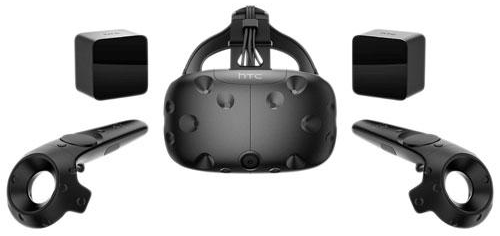
\includegraphics[width=10cm]{Images/htc-base.png} 
\caption[HTC VIVE mit VR-Brille, Controllern und Base.]{ HTC VIVE mit VR-Brille, Controllern und Base\cite{vive19}. }
\label{htc-base} 
\end{figure}


Head-Mounted Display (siehe Abbildung \ref{vr-brille}) ist ein auf den Kopf getragenes visuelles Ausgabegerät, gewöhnlich nennen wir es VR-Brille und es wird mit einem PC über einen USB-Anschluss verwendet.
Es bietet dem Benutzer ein Sichtfeld von 110$^\circ$ und einer Auflösung von 2160 x 1200 Pixeln pro Auge um die visuelle Immersion durch vollständiges Eintauchen in die virtuelle Realität ermöglichen. 
Die Bildwiederholrate von 90 Hz ermöglicht eine vollkommen natürliche ruckelfreie Wahrnehmung von Szenen und Bewegungsabläufen. 
Damit der Benutzer das Relief wahrnehmen kann, verwendet der Helm stereoskopisches Sehen, das darin besteht, unsere beiden Augen zu benutzen, um das Relief wahrzunehmen, denn Sie wissen, dass wir mit beide Augen ein  Bild unterschiedlich wahrnehmen, das Bild des rechten Auges wird im Vergleich zu dem des linken Auges verschoben und umgekehrt. 
Dieser Unterschied liegt darauf, dass unsere Augen 65 mm voneinander entfernt sind und daher nicht an der gleichen Stelle auf unserem Gesicht stehen, was zu einer Verschiebung des wahrgenommenen Bildes führt. 
Das Headset verfügt über viele Sensoren wie z.B. einen Gyroskop, (um den Benutzer im Weltraum zu lokalisieren), ein Beschleunigungsmesser und ein Laser-Positionsmesser-System. \\


\begin{figure}[h] \centering
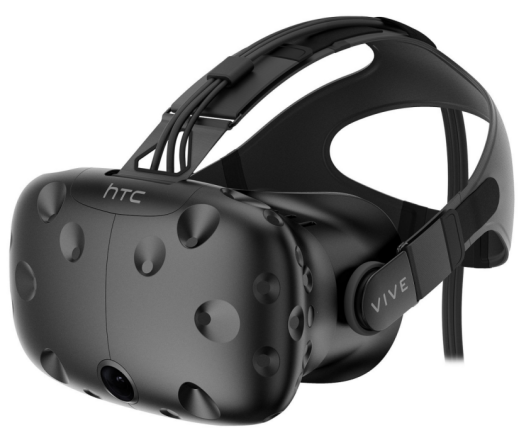
\includegraphics[width=5cm]{Images/vr-brille.png} 
\caption[VR-Brille]{ VR-Brille\cite{vive19}. }
\label{vr-brille} 
\end{figure}


Um die Position des Benutzers in einem Raum zu ermittelt, bietet das HTC VIVE zwei sogenannte ``Steam-VR-Basisstationen'' (siehe Abbildung \ref{vr-base})dem sogenannten Lighthouse-System (eine von Valve entwickelte Tracking-Technologie). 
Die Position wird dabei mit Hilfe von Infrarot-Lasern bestimmt. 
Jede Basisstation sendet Laserstrahlen aus, die von VR-Brille-Photosensoren und den Controllern erkannt werden. \\


\begin{figure}[h] \centering
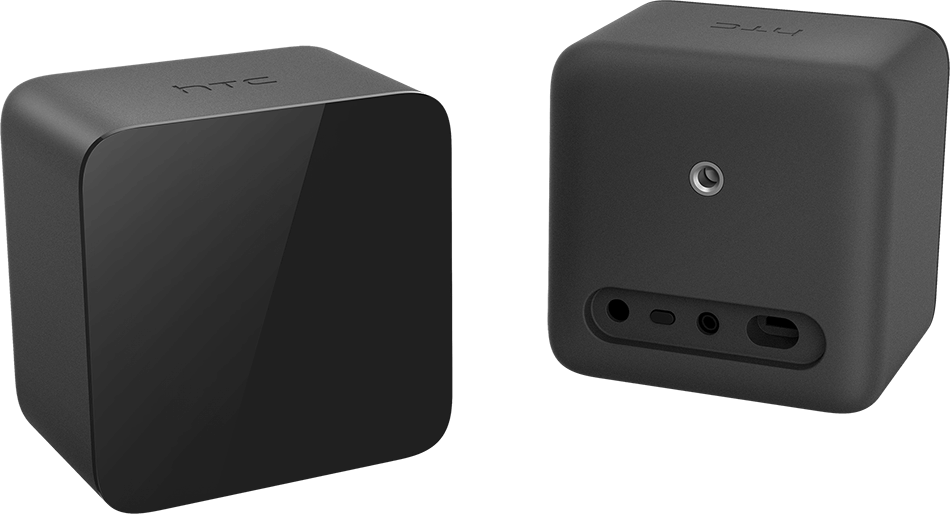
\includegraphics[width=6cm]{Images/vr-base.png} 
\caption[VR-Basisstation]{ VR-Basisstation\cite{vive19}. }
\label{vr-base} 
\end{figure}


Für eine gute Interaktion mit dem virtuellen Umgebung verfügt der Benutzer über zwei  drahtlose Controller (jeweil ein pro Hand). 
Beide drahtlosen Steuerungen sind mit Gyroskop, Beschleunigungssensor und Laserpositionssensoren. 
Die Positionsmessung der Controller erfolgt wie bei der VR-Brille über  Photosensoren. \\


\begin{figure}[h] \centering
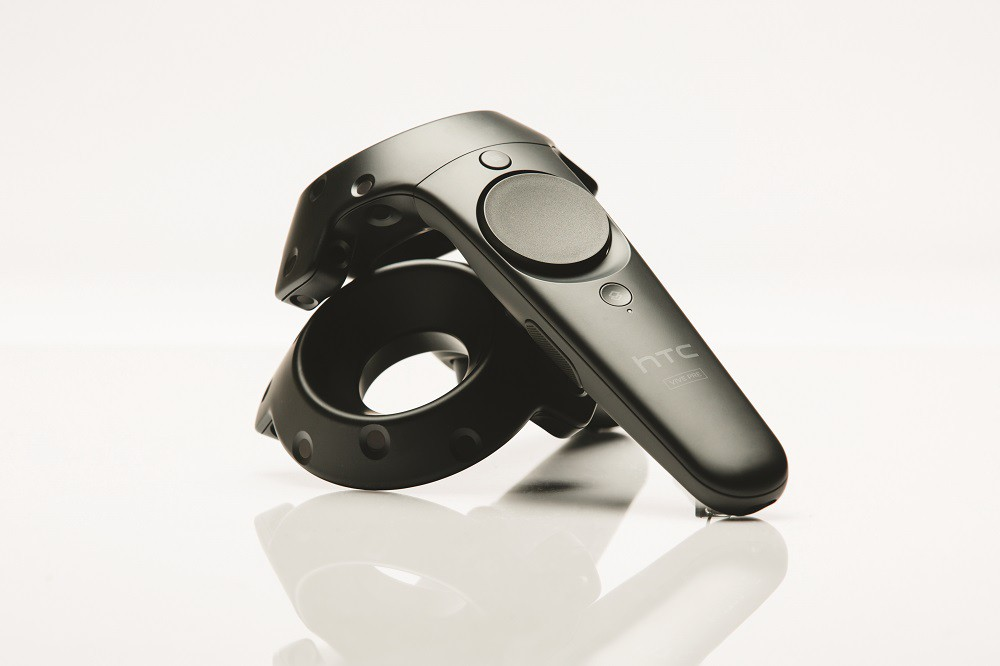
\includegraphics[width=8cm]{Images/vr-controller.png} 
\caption[VR-Controller]{ VR-Controller\cite{vive19}. }
\label{vr-controller} 
\end{figure}




\subsection{Software: Unreal engine 4} \label{vr-software}

Um unsere virtuelle Umgebung zu erzeugen, werden wir als Entwicklungsumgebung Unreal Engine verwenden. 
Unreal Engine ist eine von Epic Games entwickelte Videospiel-Engine, die sich hauptsächlich an First-Person-Shooter-Spielen orientiert, obwohl sie immer vielfältiger wird. 
Eine Spiel-Engine ist ein spezielles Framework für Computerspiele, das den Spielverlauf steuert und für die visuelle Darstellung des Spielablaufes verantwortlich ist. 
In der Regel werden derartige Plattformen auch als Entwicklungsumgebung genutzt und bringen dafür auch die nötigen Werkzeuge mit. 
Die Hauptkonkurrenten dieses Motors sind Unity, die von Crytek entwickelte CryENGINE sowie Amazon's Lumberyard (Gabel der CryENGINE). 
Unreal Engine würde von Anfang für das Projekt ELISE ausgewählt, deswegen müssten wir weiter verwenden. 
Diese Umgebung wird ständig verbessert, wir verwenden die vierte Version: Unreal Engine 4. 
Die Fähigkeiten der Unreal Engine 4 sind fantastisch. 
Es ist schon lange her, dass man dachte, die Entwicklung von Videospielen sei nur für eine Elitegruppe. 
Von nun an kann jeder Videospiele entwickeln, dank der Entwicklung von sehr zugänglichen Spiele-Engines wie der Unreal Engine 4. 
Die Unreal Engine 4 ist nicht nur extrem einfach zu bedienen und wird zunehmend von unabhängigen Studios verwendet, sondern ist auch eine der beliebtesten Spiele-Engines der größten Videospielstudios. \\

Es gibt viele Online-Tutorials, die detailliert erklären, wie Sie mit Unreal Engine beginnen können, so dass wir dieses Problem nicht untersuchen werden. 
Wir werden jedoch einige sehr wichtige Elemente (Blueprint) vorstellen, die wir während dieses Projekts verwenden werden. \\

Blueprint ist ein Programmiersystem, das als Visual Scripting System oder ``Visual Scripting'' auf Englisch bezeichnet wird. 
Eine der Besonderheiten von Unreal Engine ist der Wunsch, für alle zugänglich zu sein. 
Der Blueprint muss es denen, die nicht wissen, wie man programmiert (Zeilen Code schreibt), ermöglichen, mit der unreal Engine zu arbeiten. 
Mit Blueprint verbinden Sie einfach Elemente und lassen sie mit Visual Scripting miteinander interagieren. 
Dies ermöglicht es Ihnen, das Gleiche wie Programmierer zu tun, ohne eine Zeile Code zu schreiben(siehe Abbildung \ref{vr-blueprint}).\\

\begin{figure}[h] \centering
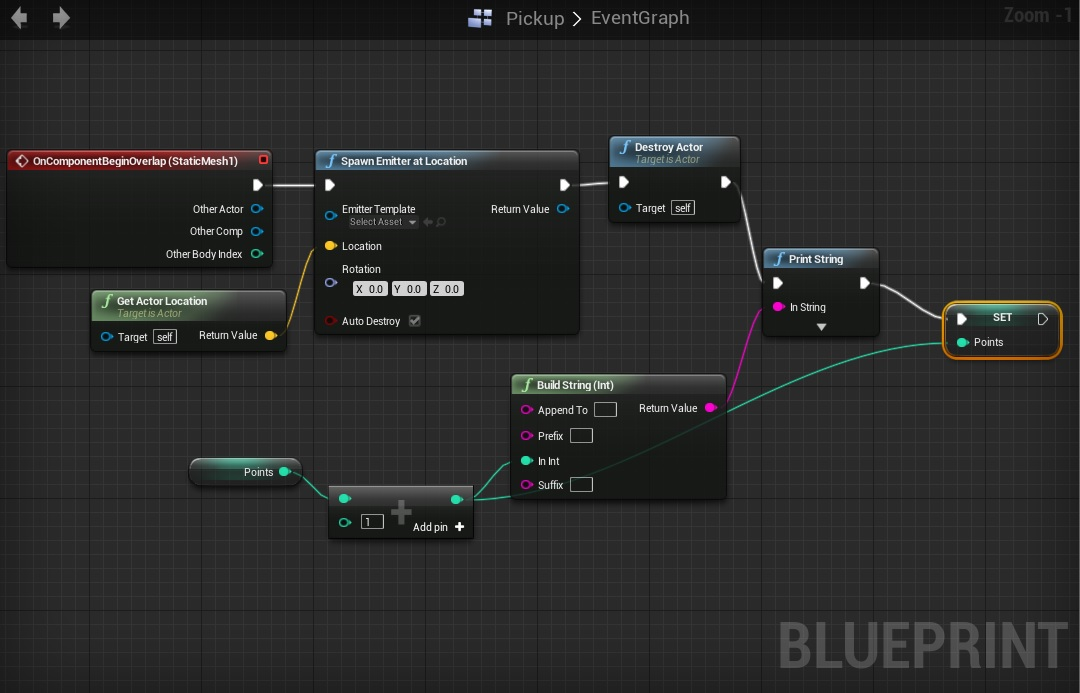
\includegraphics[width=13cm]{Images/blueprint.png} 
\caption{ Beispiel eines Blueprintcodes. }
\label{vr-blueprint} 
\end{figure}

Blueprint ist daher ein extrem leistungsfähiges System, mit dem Sie Spielprototypen sehr schnell und einfach erstellen können. 
Blueprint wurde entwickelt, um von Anfängern, Künstlern oder sogar erfahrenen Programmierern verwendet zu werden. 
Man unterscheidet LevelBlueprint und BlueprintClasse.




